%%%%%%%%%%%%%%%%%%%%%%%%%%%%%%%%%%%%%%%%%%%%%%%%%
%%%%%  make IFJtalk13.pdf
%%%%%%%%%%%%%%%%%%%%%%%%%%%%%%%%%%%%%%%%%%%%%%%%%
\documentclass{beamer}
%\documentclass[handout]{beamer}


\mode<presentation>
{
  \usetheme{Warsaw}
 %\usetheme{Hannover}
  \setbeamercovered{transparent}
}

\usepackage[english]{babel}
\usepackage{xcolor}
\usepackage[latin1]{inputenc}

\usepackage{times}
\usepackage[T1]{fontenc}
\usepackage{listings}
%------------------------------------------------------
\usepackage{amsbsy}
\usepackage{amsmath,amssymb,bbm}
\usepackage{euscript}
\usepackage{fancybox}


%%%%%%%%%%%%%%%%%%%%%%%%%%%%%%%%%%%%%%%%%%%%%%%%%%%%%%%%%%%%%%%
%%% Macros 
\newcommand{\Pcal}{{\cal P}}
\newcommand{\Kcal}{{\cal K}}
\newcommand{\Dcal}{{\cal D}}
%
\newcommand{\Peu}{\EuScript{P}}
\newcommand{\Keu}{\EuScript{K}}
\newcommand{\Deu}{\EuScript{D}}
\newcommand{\Reu}{\EuScript{R}}
\newcommand{\Feu}{\EuScript{F}}
%
\newcommand{\Pmf}{\mathfrak{P}}
\newcommand{\Dmf}{\mathfrak{D}}
%
\newcommand{\Pbbm}{\mathbbm{P}}
\newcommand{\Rbbm}{\mathbbm{R}}
\newcommand{\Zbbm}{\mathbbm{Z}}
\newcommand{\Bbbm}{\mathbbm{B}}
\newcommand{\Pop}{\overleftarrow{\Pbbm}}
\newcommand{\Zop}{\overleftarrow{\Zbbm}}
\newcommand{\Bop}{\overleftarrow{\Bbbm}}
\newcommand{\Rop}{\overleftarrow{\Rbbm}}
%
\newcommand{\Tbf}{\mathbf{T}}
\newcommand{\Pbf}{\mathbf{P}}
\newcommand{\Dbf}{\mathbf{D}}
\newcommand{\Phibf}{\mathbf{\Phi}}
%
\newcommand{\udl}{\underline}
\newcommand{\from}{\leftarrow}
\newcommand{\bu}{\bullet}
\newcommand{\veps}{\varepsilon}
\newcommand{\Dyfs}{D_{_{\rm YFS}}}
\newcommand{\tH}{{\hat{t}}}
\newcommand{\tB}{{\bar{t}}}
\newcommand{\tBl}{{\bar{t}_\lambda}}
% boldfaces and vectors
\newcommand{\ba}{{\bf{a}}}
\newcommand{\bk}{{\bf{k}}}
\newcommand{\vkap}{{\vec{\kappa}}}
\newcommand{\vrk}{{\varkappa}}
\newcommand{\alfb}{{\bar{\alpha}}}
\newcommand{\betb}{{\bar{\beta}}}


\newcommand{\cbl}{\color{blue}}
\newcommand{\crd}{\color{red}}
\newcommand{\cmg}{\color{magenta}}
\newcommand{\cgr}{\color{green}}
\newcommand{\cwh}{\color{white}}
\newcommand{\yel}{\color{yellow}}
\newcommand{\blk}{\color{black}}
\newcommand{\cya}{\color{cyan}}

\newcommand{\ns}{\normalsize}

%%%%%%%%%%%%%%%%%%%%%%%%%%%%%%%%%%%%%%%%%%%%%%%%%%%%%%%%%%%%%%%%%%%%%%%%
%%%%%%%%%%%%%%%%%%%%%%%%%%%%%%%%%%%%%%%%%%%%%%%%%%%%%%%%%%%%%%%%%%%%%%%%
%%%%%%%%%%%%%%%%%%%%%%%%%%%%%%%%%%%%%%%%%%%%%%%%%%%%%%%%%%%%%%%%%%%%%%%%
%%%%%%%%%%%%%%%%%%%%%%%%%%%%%%%%%%%%%%%%%%%%%%%%%%%%%%%%%%%%%%%%%%%%%%%%
\title[Monte Carlo Methods] % (optional)
{ {\bf MC codes for FCC-ee}
} % (optional)


\author[S.~Jadach] % (optional, use only with lots of authors)
{\Large\bf S.~JADACH }
%   \\
%   \normalsize in collaboration with B.F.L. Ward and Z. W\c{a}s}


\institute[Universities of Somewhere and Elsewhere] % (optional)
{ {\large\crd IFJ-PAN, Krak\'ow, Poland}\\
  {~~~}\\
  {\footnotesize
  Partly supported by Polish Government grant\\
  {\em Narodowe Centrum Nauki} DEC-2011/03/B/ST2/02632
}}

\date[Short Occasion] % (optional)
{\small FCC Study Kickoff Meeting\\
   Genva,
   February 15-15th, 2014
}

\subject{Talks}
% only for the PDF information catalog.

\pgfdeclareimage[height=0.5cm]{university-logo}{ifj}
\logo{\pgfuseimage{university-logo}}


\begin{document}

\begin{frame}
  \titlepage
\end{frame}
%----------------------------------------------------------------------
%----------------------------------------------------------------------
%----------------------------------------------------------------------

%----------------------------------------------------------------------
\begin{frame}[fragile]
\frametitle{\bf QED = main chalenge in Precision Measurements}

\Large\bf
In the yesterday talk by John Ellis on Physics at FCC-ee
{\cbl QED corrections} were cited as the main challenge 
{\cbl in 5 out of 9}
possible FCC-ee precision measurements.

\vspace{2mm}
In fact in 6 them:\\
$M_Z$, $\Gamma_Z$, $R_l$, 
$N_\nu \in \sigma(M_Z)$, 
$N_\nu \in \nu\bar\nu\gamma$, 
$M_W$.

\vspace{2mm}
The other 3 ones are:
$R_b$, $A_{LR}$, $M_{t}$

\end{frame}
%----------------------------------------------------------------------





%----------------------------------------------------------------------
\begin{frame}[fragile]
\frametitle{\bf QED = main chalenge in Prec. Measur. in FCCee}

\vspace{-2mm}
{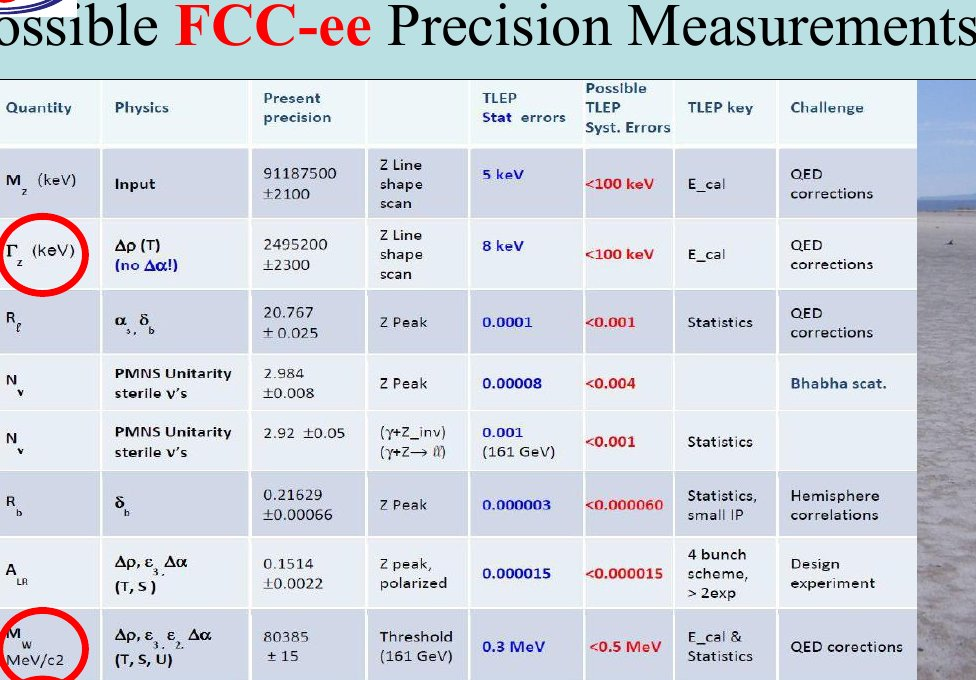
\includegraphics[width=118mm,height=85mm]{JEllis.jpg}}

\end{frame}
%----------------------------------------------------------------------

%----------------------------------------------------------------------
\begin{frame}[fragile]
\frametitle{\bf Lesson from LEP}

From LEP experience we know that\\
for the succesful mastering of the QED correction effects\\
four criteria has to be met SIMULTANEOUSLY:
\begin{enumerate}
\item
Resummation of soft photons, collienar mass logarithms,
$\ln(\Gamma/M)$, etc., to $\infty$ order, +RGE
\item
Inslusion of the SELECTED higher order Feynman diagrams,
\item
Monte Carlo implementation
\end{enumerate}


\end{frame}
%----------------------------------------------------------------------


%----------------------------------------------------------------------
\begin{frame}[fragile]
\frametitle{\bf Example of the QED Precision evolution }

\vspace{-2mm}
{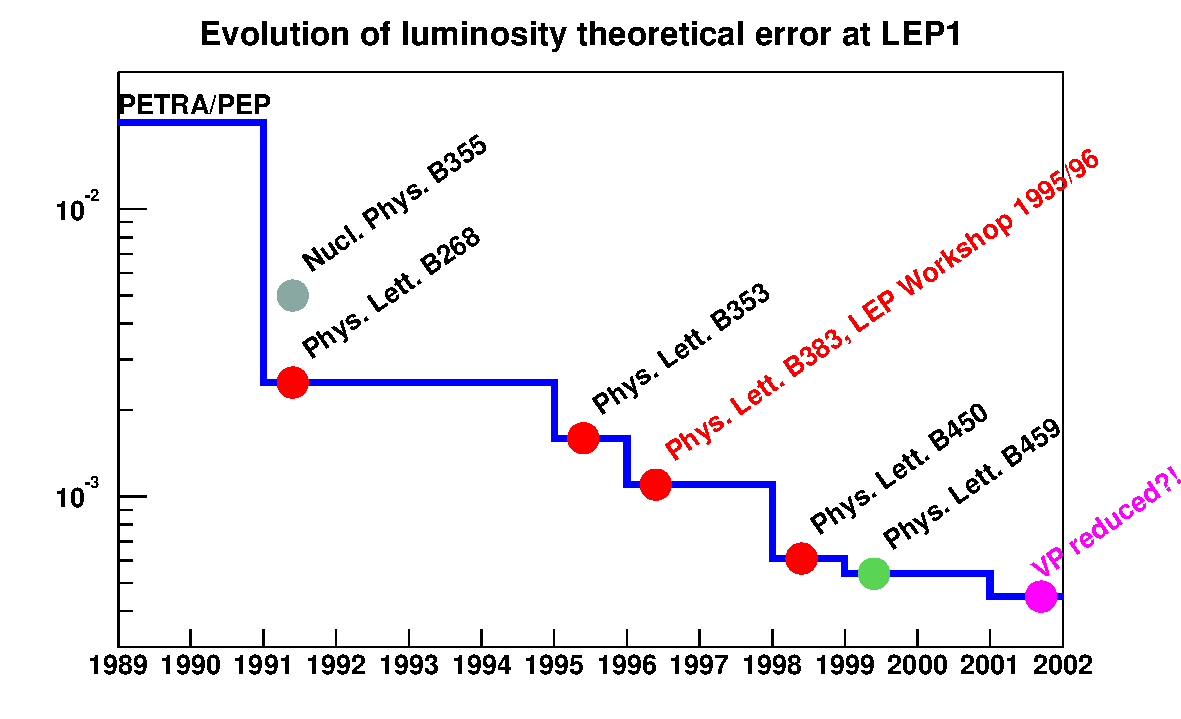
\includegraphics[width=110mm,height=80mm]{cFigA.pdf}}

\end{frame}
%----------------------------------------------------------------------



%----------------------------------------------------------------------
\begin{frame}[fragile]
\frametitle{\bf QED effects calculatios at LEP}
\Large\bf
\begin{itemize}
\item
{\cbl Non-MC QED calculations}, Z-lineshape:\\
{\ns 
NB. QED 3-rd order exponentiated formula
by S.J. and Skrzypek used in Zfitter, still teh best:)}
\item
QED in form of {\cbl MC generators}
were used for all other LEP
measurables, processes.
\end{itemize}

\end{frame}
%----------------------------------------------------------------------









%----------------------------------------------------------------------
\begin{frame}[fragile]
\frametitle{\bf MC programs from Krakow group}
\framesubtitle{\bf (with the important US component:)}

Legacy codes from LEP era which are still kept alive:

\begin{itemize}
\item
KKMC for $e^-e^+ \to f\bar{f}+ n\gamma$,\\
$f=\mu,\tau,\nu,u,d,s,c,b$,~~~~ $n=0,1,2...\infty$
\item
TAUOLA for $\tau$ decays and PHOTOS for extra photon emission
is part of KKMC and other programs
\item
BHLUMI for small angle $e^-e^+ \to e^-e^+$
\item
BHWIDE for large angle $e^-e^+ \to e^-e^+$
\item
KORALW and YFSWW for $e^-e^+ \to W^-W^+ \to 4f $
\item
YFZZZ for $e^-e^+ \to ZZ \to 4f $
\end{itemize}

\end{frame}
%----------------------------------------------------------------------


%----------------------------------------------------------------------
\begin{frame}[fragile]
\frametitle{\bf What is KKMC?}
{\large
KKMC is the MC event generator for the process:\\
~~~~~~~~~~~~~~\fbox{\cbl $e^-e^+ \to f\bar{f}+ n\gamma$}\\
{\cbl $f=\mu,\tau,\nu,u,d,s,c,b$,~~~~ $n=0,1,2...\infty$.}
}\\
Interfaced with TAUOLA+PHOTOS\\
and with electroweak library DIZET.\\

Published version \fbox{\cmg 4.13} (to be cited):
\begin{itemize}
\item
Comput.Phys.Commun. 130(2000) 360, hep-ph/9912214,\\
F77 code description and user guide (manual).
\item
Phys. Rev. D63 (2001) 113009, hep-ph/0006359\\
physics content, CEEX exponentiation of QED corrs.\\
\end{itemize}
"Workhorse" in data analysis of all four LEP collaborations.\\
~~~\\
\footnotesize
(Replacement of earlier MC's KORALZ and KORALB.)\\
(Not aplicable for  $e^-e^+ \to e^-e^+$)

\end{frame}
%----------------------------------------------------------------------

%----------------------------------------------------------------------
\begin{frame}[fragile]
\frametitle{\bf More KKMC versions available since 2000}
\framesubtitle{http://jadach.web.cern.ch/jadach/KKindex.html}
\small
\begin{itemize}
\item
Production Version \fbox{\cmg 4.16}, Oct. 2001,  
(KKMC-v.4.16d-export.tar.gz).
Improved $\nu\bar{\nu}$ matrix elm.\\
RRes module for $\gamma^* \to narrow~resonances$ at LEP.
\item
Developement Version \fbox{\cmg 4.19}, Sept. 2002,  
(KKMC-v.4.19.b-export.tar.gz). C++ wrapper.\\
Improved $\nu\bar{\nu}$ matrix element and RRes for low energy colliders.\\
ISR with complete NLO corrs,
as in Phys.Rev. D65(2002) 073030 by S.J., M.Mells, B.F.L.Ward and S.A. Yost.\\
Collinear beamstrahlung for NLC/ILC.
\item
{\cbl
Developement Version \fbox{\cmg 4.22}, June 2013,  
(KKMC\_v4\_22.tgz).
Tested $\mu^-\mu+$ and $q\bar{q}$ beams
(instead of $e^-e^+$) at fixed energy.
Optionaly, collinear PDFs for $q\bar{q}$ beams instead of beamstrahlung,
as a patch in the source code (temp. solution).}
\item
{\footnotesize
The complete "algebraic" description of the NNLO formulas has been
published in Phys.Rev. D73 (2006) 073001
(an extension of the work in Phys.Rev. D65 (2002) 073030),
the code still not public.\\
PHOKHARA MC is an alternative here for low energy colliders.}
\end{itemize}


\end{frame}
%----------------------------------------------------------------------

%----------------------------------------------------------------------
\begin{frame}[fragile]
\frametitle{\bf Hidden treasures in KKMC}
\framesubtitle{Can be useful for LHC?}
\small
KKMC is special because:
\begin{itemize}
\item
Resummed (exponentiated) multiphoton effects at the AMPLITUDE level (CEEX).
$\sim$10 man-years of work in QED.
\item
QED rad. corrections up to third LO and NLO, both in the initial
and final state plus (exponentiated) initial-final interference.
\item
Complete spin effects, including transverse correlations, for incoming beams
and outgoing femions (needed for taus).
\end{itemize}

\footnotesize
KKMC can be useful in the LHC data analysis,\\
without major developments beyond the existing code:
\begin{itemize}
\item
Testing/calibrating PHOTOS for FSR in leptonic decays of Z/W.\\
An obvious thing and Zbyszek Was is doing this all the time...
\item
Studies/estimations of ISR-FSR interferences in 
$q\bar{q} \to Z \to l+\bar{l}$ data
\item
Electroweak+QCD corrections in the for Z production.cross section
\item
Spin correlations in $Z \to \tau^-\tau^+$, already being done by Zbyszek
\item
What else???? Any new ideas????
\end{itemize}

\end{frame}
%----------------------------------------------------------------------


%----------------------------------------------------------------------
\begin{frame}[fragile]
\frametitle{\bf More on KKMC version 4.22 (2013)}
\framesubtitle{\bf\large Technical points}
\small
\begin{itemize}
\item
Old benchmarks, Table III in Pys.Rev. D 63 (2001) and more,
are reproduced under SLC5 and SLC6, 
after adjustments of flags in makefile's
and minor corrections in f77 code.
\item
Unpublished (public) v.4.16,4.19 include varying subset of extra subdirectories,
not included in v4.13. Also not in v.4.22.
\item
System of original interrelated custom $Makefile$'s 
is renamed $Makefile\to KKMakefile$
and preserved.
\item
$Atomake/Autotools$ are introduced ($makefile.am$ etc.).\\
Hence KKMC is more platform independent\\
and can be easily put under $kdevelop3$ or $eclipse$.
\item
Interface to C++ is provided.
Main program (histogramming, etc) can be in C++, using optionally ROOT.
(On request, or in v4.19)
\item
Scripts for running on PC-farms slightly upgraded and working.
\item
Old versions of PHOTOS and TAUOLA.
\end{itemize}
\end{frame}
%----------------------------------------------------------------------



\end{document}
%%%%%%%%%%%%%%%%%%%%%%%%%%%%%%%%%%%%%%%%%%%%%%%%%%%%%%%%%%%%%%%%%%%%%%%%
%%%%%%%%%%%%%%%%%%%%%%%%%%%%%%%%%%%%%%%%%%%%%%%%%%%%%%%%%%%%%%%%%%%%%%%%
%%%%%%%%%%%%%%%%%%%%%%%%%%%%%%%%%%%%%%%%%%%%%%%%%%%%%%%%%%%%%%%%%%%%%%%%
%%%%%%%%%%%%%%%%%%%%%%%%%%%%%%%%%%%%%%%%%%%%%%%%%%%%%%%%%%%%%%%%%%%%%%%%


%----------------------------------------------------------------------
\begin{frame}[fragile]
\frametitle{Abstract (plan of the talk)}
%\framesubtitle{Mission statement}
...
\end{frame}
%----------------------------------------------------------------------


